\documentclass[../main.tex]{subfiles}
\begin{document}
\chapter{Linear PDEs and Separation of Variables}
\section{Boundary and Initial Value Problems}
\subsection{Definition}
We are interested in solving both \textit{pure boundary value problems} (abbreviated as \textit{BVP}) and \textit{initial boundary value problems} (abbreviated as \textit{IBPV}).

\begin{remark}[Recap]
  Recall from IA Vector Calculus that for a region $\Omega$ of $\R^n$ for $n \in \{1, 2, 3\}$, we denote its boundary as $\partial \Omega$.
\end{remark}
Let $P$ and $Q$ be \textit{linear partial differential operators} and let $\Omega \subseteq \R^n$ be open, bounded, and connected.
In this course, we will only consider $n \in \{1, 2, 3\}$.

Pure boundary value problems are PDEs for a function of space on some region $\Omega$ and as such only have boundary conditions on $\partial \Omega$:
\[
  \begin{cases}
  P\varphi(\vec{x}) = 0 & \text{ for } \vec{x} \in \Omega \\
  \text{Boundary conditions} & \text{ for } \vec{x} \in \partial \Omega
  \end{cases}
\]
Initial boundary value problems are PDEs for a function of both space and time on some region $\Omega$ and interval of time $[0, T)$.
These have both boundary conditions on $\partial \Omega$ and an \textit{initial condition} at $t = 0$:
\[
  \begin{cases}
  Q \varphi(\vec{x}, t) = 0 & \text{ for } (\vec{x}, t) \in \Omega \times (0, T) \\
  \text{Boundary conditions} & \text{ for } (\vec{x}, t) \in \partial \Omega \times (0, T) \\
  \text{Initial conditions} & \text{ for } (\vec{x}, t) \in \Omega \times \{0\}
  \end{cases}
\]

\subsection{Splitting up IBVPs}
IBVPs can have quite a few boundary and initial conditions so it is useful to note that we can use linearity to split such problems up into two separate problems.

For example, we could split it into zero and non-zero boundary/initial conditions:
\begin{align*}
  &\begin{cases}
  Q \varphi_1(\vec{x}, t) = 0 & \text{ for } (\vec{x}, t) \in \Omega \times (0, T) \\
  \text{All B.C.s} = 0 & \text{ for } (\vec{x}, t) \in \partial \Omega \times (0, T) \\
  \text{Remaining I.C.s} & \text{ for } (\vec{x}, t) \in \Omega \times \{0\}
  \end{cases} \\
  &\begin{cases}
  Q \varphi_2(\vec{x}, t) = 0 & \text{ for } (\vec{x}, t) \in \Omega \times (0, T) \\
  \text{Remaining B.C.s} & \text{ for } (\vec{x}, t) \in \partial \Omega \times (0, T) \\
  \text{All I.C.s = 0} & \text{ for } (\vec{x}, t) \in \Omega \times \{0\}
  \end{cases}
\end{align*}
Using the linearity of $Q$, $\varphi = \varphi_1 + \varphi_2$ solves the original problem.
We can split the boundary/initial conditions in any way provided that $\phi_1 + \phi_2$ satisfies those from the original problem.
\subsection{Convenient Domains}
In this course, we will only consider problems defined on a domain $\Omega$ which is able to be transformed into a line/rectangle/cuboid (depending on $n$) by performing a change of variables.
Thus from now on we will assume that $\Omega$ is a line/plane/rectangle.

In this case, we can further assume without loss of generality that all boundary conditions vanish on all but one endpoint/edge/face.
This is best demonstrated using an example.
\begin{example} \label{domainSplitEx}
  Consider the BVP on the square $\Omega = (0, 1) \times (0, 1)$:
  \[
    \begin{cases}
    P \psi = 0 & \text{ for } (x, y) \in (0, 1) \times (0, 1) \\
    \psi = f_i & \text{ on the $i$-th side}
    \end{cases}
  \]
  We split this into four separate problems for $\psi_i$, $i \in \{1, 2, 3, 4\}$:
  \[
    \begin{cases}
    P \psi_i = 0 & \text{ for } (x, y) \in (0, 1) \times (0, 1) \\
    \psi_i = f_i & \text{ on $i$-th side} \\
    \psi_i = 0 & \text{ not on the $i$-th side}
    \end{cases}
  \]
  These problems have a zero boundary condition on all but one side as stipulated.
  By linearity of $Q$, $\psi = \psi_1 + \psi_2 + \psi_3 + \psi_4$ solves the original problem and so we solve each of these problems separately.

  Pictorially, this is:
  \begin{center}
  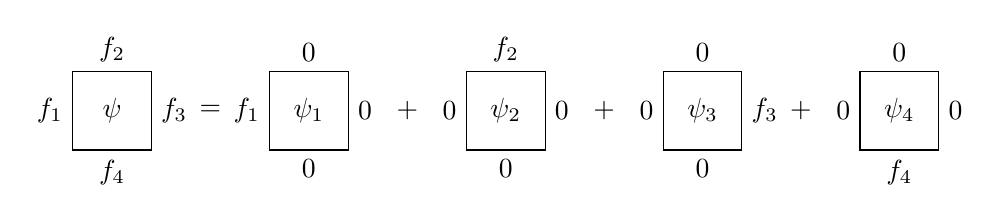
\begin{tikzpicture}
    \begin{scope}[scale=0.5]
      \draw (-1, -1) -- node[left] {$f_1$} (-1, 1) -- node[above] {$f_2$} (1, 1) -- node[right] {$f_3$} (1, -1) -- node[below] {$f_4$} cycle;
      \node at (0, 0) {$\psi$};
      \node at (2.5, 0) {$=$};
    \end{scope}
    \begin{scope}[scale=0.5, xshift=5cm]
      \draw (-1, -1) -- node[left] {$f_1$} (-1, 1) -- node[above] {$0$} (1, 1) -- node[right] {$0$} (1, -1) -- node[below] {$0$} cycle;
      \node at (0, 0) {$\psi_1$};
      \node at (2.5, 0) {$+$};
    \end{scope}
    \begin{scope}[scale=0.5, xshift=10cm]
      \draw (-1, -1) -- node[left] {$0$} (-1, 1) -- node[above] {$f_2$} (1, 1) -- node[right] {$0$} (1, -1) -- node[below] {$0$} cycle;
      \node at (0, 0) {$\psi_2$};
      \node at (2.5, 0) {$+$};
    \end{scope}
    \begin{scope}[scale=0.5, xshift=15cm]
      \draw (-1, -1) -- node[left] {$0$} (-1, 1) -- node[above] {$0$} (1, 1) -- node[right] {$f_3$} (1, -1) -- node[below] {$0$} cycle;
      \node at (0, 0) {$\psi_3$};
      \node at (2.5, 0) {$+$};
    \end{scope}
    \begin{scope}[scale=0.5, xshift=20cm]
      \draw (-1, -1) -- node[left] {$0$} (-1, 1) -- node[above] {$0$} (1, 1) -- node[right] {$0$} (1, -1) -- node[below] {$f_4$} cycle;
      \node at (0, 0) {$\psi_4$};
    \end{scope}
  \end{tikzpicture}
  \end{center}
\end{example}
\begin{remark}[Advice]
  Linearity is one of the only inherent properties of BVPs and so it is important to utilise it.
\end{remark}
\section{Laplace's Equation}
\subsection{Definitions}
Recall Laplace's equation from IA Vector Calculus.
\begin{definition}[Laplace's Equation]
  For $\varphi: \R^n \to \R$, \textit{Laplace's equation} is:
  \[
    \Delta \phi = 0
  \]
  where $\Delta = \nabla \cdot \nabla$ is the \textit{Laplacian}
\end{definition}
\begin{remark}[Notation]
  This is the same Laplacian as in IA Vector Calculus however we now use the notation $\Delta$ instead of $\nabla^2$.
\end{remark}
\begin{remark}[Intuition]
  $\Delta \varphi(\vec{x})$ measures the extent to which $\varphi(\vec{x})$ differs from its average over an infinitesimal region centered at $\vec{x}$.
  So if $\Delta \varphi(\vec{x}) = 0$, then $\varphi$ agrees with its nearby averages, suggesting that there is a state of equilibrium.
\end{remark}
\begin{definition}[Harmonic function]
  We say that $\varphi$ is \textit{harmonic} if $\Delta \varphi = 0$ on its entire domain.
\end{definition}
\begin{example}[Imcompressible and irrotational flow]
  Let $\vec{u}: \R^3 \to \R^3$ be the velocity of an incompressible and irrotational fluid.
  Since it is incompressible, $\nabla \cdot \vec{u} = \vec{0}$, and since it is irrotational $\nabla \times \vec{u} = \vec{0}$.

  We saw in IA Vector Calculus, that since $\vec{u}$ is irrotational and $\R^3$ is a simply connected domain, there exists a scalar potential $\varphi: \R^3 \to \R$ such that $\vec{u} = \nabla \varphi$.
  Thus incompressibility tells us that $\Delta \vec{u} = \nabla \cdot \nabla \vec{u} = 0$ and so $\vec{u}$ is harmonic.
\end{example}
To obtain a pure BVP, we need to impose boundary conditions:
\[
  \begin{cases}
  \Delta \varphi(\vec{x}) = 0 & \text{ if } \vec{x} \in \Omega \\
  B\varphi(\vec{x}) = f(\vec{x}) & \text{ if } \vec{x} \in \partial \Omega
  \end{cases}
\]
for a linear differential operator $B$.

As in IA Vector Calculus, we will consider two types of boundary conditions:
\begin{itemize}
  \item \textit{Dirichlet} boundary conditions, these have $B \varphi \equiv \phi$.
  \item \textit{Von-Neumann} boundary conditions, these have $B \varphi \equiv \pderiv{\varphi}{\vec{n}}$
\end{itemize}
\begin{remark}[Recap]
  Recall from IA Vector Calculus the notation:
  \[
    \pderiv{}{\vec{n}} = \vec{n} \cdot \nabla
  \]
  where $\vec{n}(\vec{x})$ is the outwards normal to $\Omega$ at $\vec{x} \in \partial \Omega$.

  Moreover, recall that in the case of Dirichlet boundary conditions, solutions to such BVP are unique, and in the case of Von-Neumann, solutions are unique up to an additive constant.
\end{remark}
\subsection{Separation of Variables on a Square} \label{sepSquare}
Suppose we want to the following BVP for Laplace's equation on the square $\Omega = (0, 1) \times (0, 1)$.
\[
  \begin{cases}
  \varphi_{x x} + \varphi_{y y} = 0 & \text{ for } (x, y) \in (0, 1) \times (0, 1) \\
  \varphi(x, y) = 0 & \text{ for } x \in \{0, 1\} \text{ or } y = 0 \\
  \varphi(x, 1) = f(x) &  \text{ for } x \in (0, 1)
  \end{cases}
\]
We first consider the homogeneous part of the problem:
\[
  \begin{cases}
  \Delta \varphi = \varphi_{x x} + \varphi_{y y} = 0 & \text{ for } (x, y) \in (0, 1) \times (0, 1) \\
  \varphi(x, y) = 0 & \text{ for } x \in \{0, 1\} \text{ or } y = 0 \\
  \end{cases}
\]
We can use \textit{separation of variables} to look for a solution to this.
To do this, we guess that the solution is of the form $\varphi = X(x)Y(y)$.
Substituting this into $\Delta \varphi = 0$, we obtain:
\[
  \frac{X''(X)}{X(x)} + \frac{Y''(y)}{Y(y)} = 0 \implies \frac{X''(x)}{X(x)} = - \frac{Y''(y)}{Y(y)}
\]
Since both sides depend only on different variables, there must exist some constant $\lambda \in \R$ such that:
\[
  X'' + \lambda X = 0 \text{ and } Y'' - \lambda Y = 0
\]
For the homogeneous problem we want $\varphi = 0$ when $x \in \{0, 1\}$, the problem for $X$ is:
\[
  \begin{cases}
  -X'' = \lambda X & \text{ for } x \in (0, 1) \\
  X(0) = 0 &  \\
  X(1) = 0 &
  \end{cases}
\]
This is the Sturm-Liouville problem we saw in \cref{slpExample} with $L = 1$!
Thus the eigenfunctions of this problem are:
\[
  X_n(x) = \sin(n \pi x) \text{ for } n \in \N
\]

$Y$ also must solve a particular Sturm-Liouville problem.
In this case the eigenfunctions are:
\[
  Y_n(y) = \sinh (n \pi y) \text{ for } n \in \N
\]

Since scaled eigenfunctions are still eigenfunctions, we can scale $X_n$ and $Y_n$ by arbitrary constants for each $n$.
Thus the homogeneous part of the problem is satisfied by:
\[
  \varphi_n(x, y) = A_n \sin(n \pi x)\sinh(n \pi y)
\]
for $n \in \N$ where $A_n$ is an arbitrary constants.

Since this is for the homogeneous problem and the problem is linear, the superposition of arbitrarily many solutions solves and so:
\[
  \varphi(x, y) = \sum_{n = 0}^{\infty} A_n \sin(n \pi x)\sinh(n \pi y)
\]
also solves the homogeneous problem.

For it to satisfy the inhomogeneous boundary condition, we need:
\[
  f(x) = \varphi(x, 1) = \sum_{n = 1}^{\infty} A_n \sin(n \pi x) \sinh(n \pi)
\]
Can we pick the coefficients $A_n$ in such a way that this holds?

Since $\{X_n\}$ are eigenfunctions of a Sturm-Liouville problem with $w = 1$, they satisfy an orthogonality relation:
\[
  \langle X_n, X_m \rangle = \int_{0}^{1} \sin(n \pi x) \sin(m \pi x) \d{x} = \frac{1}{2} \delta_{n m}
\]
Suppose now that the boundary condition is satisfied, i.e. $f(x) = \varphi(x, 1)$ for $x \in (0, 1)$.
Thus when we take the inner product of $f(x) = \psi(x, 1)$ with $X_m$ we obtain:
\begin{align*}
  \langle f, X_m \rangle &= \sum_{n = 1}^{\infty} A_n \langle X_n, X_m \rangle \sinh(n \pi) \\
                         &= \frac{1}{2} A_m \sinh(n \pi)
\end{align*}
For $n \in \N$, $\sinh(n\pi) > 0$ and so we can take the coefficients as:
\[
  A_n = \frac{2}{\sinh(n \pi)} \langle f,X_m \rangle = \frac{2}{\sinh(n \pi)} \int_{0}^{1} f(x) \sin(n \pi x) \d{x}
\]
Thus with these coefficients, the function $\varphi$ given by:
\[
  \varphi(x, y) = \sum_{n = 1}^{\infty} A_n \sin(n \pi x)\sinh(n \pi y)
\]
solves the full BVP.
\begin{remark}
  When we impose a boundary condition, we do not just mean that the boundary condition is satisfied exactly on the boundary but implicitly that solutions continuously approach these boundary conditions from inside the domain.
  We did not checked that was is necessarily the case in the above example, however, we shall not worry about such details within this course.
\end{remark}
\subsection{Separation of Variables an Circular Annulus}
We would like to solve Laplace's equation on the annular region $r_1 < |\vec{x}| < r_2$ in $\R^2$.
It is therefore convenient to use polar coordinates $(r, \theta)$ so that the annular region in the $x$-$y$ plane becomes a rectangular region in the $r$-$\theta$ plane.

In IA Vector calculus, we saw that Laplace's equation in polar coordinates is:
\[
  \frac{1}{r} \pderiv{}{r}\left(r \pderiv{\varphi}{r}\right) + \frac{1}{r^2} \pderiv[2]{\varphi}{\theta} = 0
\]
Since we are just solving this on a rectangular region in the $r$-$\theta$ plane, we apply a similar method as we did in \cref{sepSquare}.

We look for a separable solution of the form $\varphi = R(r) \Theta(\theta)$.
Upon substituting in, we obtain:
\[
  \frac{r}{R} \deriv{}{r}\left[r \pderiv{R}{r}\right] + \frac{1}{\Theta} \pderiv[2]{\Theta}{\theta} = 0 \implies \frac{r}{R} \deriv{}{r}\left[r \pderiv{R}{r}\right] = - \frac{1}{\Theta} \pderiv[2]{\Theta}{\theta}
\]
The left hand side of this depends only on $r$ and the right hand side depends only on $t$, thus, there exists $\lambda \in \R$ such that:
\[
  \Theta'' + \lambda \Theta = 0 \text{ and } r(rR')' = \lambda R
\]
\subsubsection{Solving for $\Theta$}
Considering $\Theta'' + \lambda \Theta = 0$, for $\lambda \neq 0$, we obtain:
\[
  \Theta(\theta) = A \cos(\sqrt{\lambda} \theta) + B \sin(\sqrt{\lambda} \theta)
\]
Due to the circular symmetry, we must have  $\varphi(r, \theta) = \varphi(r, \theta + 2\pi)$ for all $\theta$, and so $\lambda = n^2$ for some $n \in \N_0$.

\subsubsection{Solving for $R$}
Using our expression for $\lambda$, we then have $r(rR')' = n^2 R$.
The left hand side of this has equally $r$ as it does derivatives, so if $n \neq 0$, we try to look for a solution of the form $R = r^\alpha$.
Upon substituting this in, we obtain $\alpha = n^2$, i.e. $r^\alpha$ solves for $\alpha = \pm n$.

In the case of $n =0$, we obtain $R = A + B \log r$.

\subsubsection{Family of Solutions}
By linearity, we obtain a family of solutions of the form:
\[
  \phi(r, \theta) = A + B \log r + \sum_{n = 1}^{\infty} [A_n r^n + B_n r^{-n}][C_n \cos(n\theta) + D_n \sin(n \theta)]
\]
for arbitrary constants $A_n, B_n, C_n, D_n$.
\begin{remark}
  If the domain contains $r = 0$, then we must have $B = 0$ and $B_n = 0$ for all $n \geq 1$.
\end{remark}
\begin{example}
  Suppose we want to solve the following:
  \[
    \begin{cases}
    \Delta \varphi = 0 & \text{ for } r_1 < r < r_2 \\
    \varphi = 0 & \text{ for }r = r_1 \\
    \varphi = f(\theta) & \text{ for } r = r_2
    \end{cases}
  \]
  Define the following:
  \[
    R_0(r) = A + B \log r \text{ and } R_n(r) = A_n r^{n} + B_n r^{-n} \text{ for } n \geq 1
  \]
  Looking at the analysis above, if we enforce $R_n(r_1) = 0$, then for $n = 0$:
  \[
    R_0(r_1) = A + B \log r_1 = 0 \implies A = -B \log r_1 \implies R_0(r) = C_0 \log \left(\frac{r}{r_1}\right)
  \]
  where we redefine the constant $B = C_0$.
  For $n \geq 1$:
  \[
    R_n (r_1) = A_n r^{n}_{1} + B_n r^{-n}_{1} = 0 \implies A_n = -B_n r^{-2n} \implies R_n(r) = C_n \left[\left(\frac{r}{r_1}\right)^n - \left(\frac{r_1}{r}\right)^{n}\right]
  \]
  where we redefine $B_n = C_n r^{n}_{1}$.

  Thus, our family of solutions from earlier becomes:
  \[
    \varphi(r, \theta) = C_0 \log\left(\frac{r}{r_1}\right) + \sum_{n = 1}^{\infty} \left[\left(\frac{r}{r_1}\right)^n - \left(\frac{r_1}{r}\right)^{n}\right][C_n \cos(n\theta) + D_n \sin(n \theta)]
  \]
  We also want that at $r = r_2$:
  \[
    f(\theta) = C_0 \log\left(\frac{r_2}{r_1}\right) + \sum_{n = 1}^{\infty} \left[\left(\frac{r_2}{r_1}\right)^n - \left(\frac{r_1}{r_2}\right)^{n}\right][C_n \cos(n\theta) + D_n \sin(n \theta)]
  \]
  This looks quite similar to a Fourier series.
  In fact, if we define:
  \begin{align*}
    \frac{1}{2} a_0 &= C_0 \log\left(\frac{r_2}{r_1}\right) \\
    \text{ and } a_n &= \left[\left(\frac{r_2}{r_1}\right)^n - \left(\frac{r_1}{r_2}\right)^{n}\right]C_n \\
    \text{ and } b_n &= \left[\left(\frac{r_2}{r_1}\right)^n - \left(\frac{r_1}{r_2}\right)^{n}\right]D_n
  \end{align*}
  then:
  \[
    f(\theta) = \frac{1}{2} a_0 + \sum_{n = 1}^{N} [a_n \cos(n\theta) + b_n \sin(n\theta)]
  \]
  This is a Fourier series as we saw in \label{fourierChap}!
  Thus we can compute $a_n$ and $b_n$ from $f$ using:
  \[
    a_n = \frac{1}{\pi} \int_{0}^{2\pi} f(\theta) \cos(n\theta) \d{\theta} \text{ and } b_n = \frac{1}{\pi} \int_{0}^{2\pi} f(\theta) \sin(n\theta) \d{\theta}
  \]
  We can then use this to find the coefficients $C_n$ and $D_n$ to construct the final $\varphi(r, \theta)$.
  Since this solves and the boundary conditions are Dirichlet B.C.s, it is \textit{the} solution to the problem by uniqueness.

  If we wanted to instead solve with a boundary function at both $r_1$ and $r_2$, that is:
  \[
    \begin{cases}
    \Delta \varphi = 0 & \text{ for } r_1 < r < r_2 \\
    \varphi = f_1(\theta) & \text{ for }r = r_1 \\
    \varphi = f_2(\theta) & \text{ for } r = r_2
    \end{cases}
  \]
  then we can use the method from \cref{domainSplitEx} to find $\varphi_1$ and $\varphi_2$ which each solve with only one functional boundary condition and one zero boundary condition so that $\varphi = \varphi_1 + \varphi_2$ solves this problem.
\end{example}
\subsection{Separation of Variables on Spherical Annulus}
We would also like to solve Laplace's equation on the spherical annulus $r_1 < |\vec{x}| < r_2$ but in $\R^3$.
Similarly in in $\R^2$, it makes sense to use spherical polars $(r, \theta, \phi)$, where $r$ is the radial coordinate, $\theta \in [0, \pi]$ and $\varphi \in [0, 2\pi]$.

For ease, we assume that the solution is symmetric about the $z$-axis, so $\varphi = \varphi(r, \theta)$.

In IA Vector Calculus, we saw that Laplace's equation in spherical polars is:
\[
  \frac{1}{r^2} \pderiv{}{r}\left[r^2 \pderiv{\varphi}{r}\right] + \frac{1}{r^2 \sin \theta} \pderiv{}{\theta}\left[\sin \theta \pderiv{\varphi}{\theta}\right] + \frac{1}{r^2 \sin^2 \theta} \cancelto{0}{\pderiv[2]{\varphi}{\phi}} =0
\]
Similarly, we try to find a separable solution $\varphi = R(r)\Theta(\theta)$.
Upon substituting this in we obtain:
\[
  \frac{1}{R} \deriv{}{r}\left[r^2 \deriv{R}{r}\right] + \frac{1}{\Theta \sin \theta} \deriv{}{\theta}\left[\sin \theta \pderiv{\Theta}{\theta}\right] = 0
\]
As we did previously, there must exist $\lambda \in \R$ such that:
\[
  (r^2 R')' = \lambda R \text{ and } -[\Theta' \sin \theta]' = \lambda \Theta \sin \theta
\]
\subsubsection{Solving for $\Theta$}
In the equation for $\Theta$, we perform the substitution $x(\theta) = \cos \theta$ and write $\widetilde{\Theta}(x) = \Theta(\theta)$.
Using the chain rule:
\begin{align*}
  \pderiv{\Theta}{\theta} &= \deriv{x}{\theta} \pderiv{\widetilde{\Theta}}{x} \\
                          &= - \sin \theta \pderiv{\widetilde{\Theta}}{x} \implies \deriv{}{\theta} = - \sin \theta \deriv{}{x}
\end{align*}
Substituting this in, we obtain:
\[
  -\left(\sin \theta \deriv{}{x}\right)\left[\sin \theta\left(\sin \theta \deriv{\widetilde{\Theta}}{x}\right)\right] = \lambda \widetilde{\Theta} \sin \theta
\]
Assuming $\theta \notin \{0, \pi\}$, i.e. $-1 < x < 1$, we can divide through by $\sin \theta$ and rewrite $\sin^2 \theta = 1 - \cos^2 \theta = 1 - x^2$ to obtain:
\[
  -\deriv{}{x}\left[(1 - x^2) \pderiv{\widetilde{\Theta}}{x}\right] = \lambda \widetilde{\Theta} \text{ for } -1 < x < 1
\]
This is Legendre's equation from \cref{legendre}!
We saw that this has eigenfunctions given by:
\[
  \widetilde{\Theta} = P_n(x),\ \lambda_n = n(n + 1) \text{ for $n \in \N_0$}
\]
Transforming these back to the original coordinates, we obtain solutions for $\Theta$:
\[
  \Theta(\theta) = P_n(\cos \theta)
\]
\subsubsection{Solving for $R$}
Using our value for $\lambda_{n} = n(n + 1)$, the equation for $R$ is:
\[
  (r^2 R')' = n(n + 1) R
\]
We again try $R = r^\alpha$, and upon substituting this in, we obtain:
\[
  \alpha(\alpha + 1) = n(n + 1) \iff (\alpha - n)(\alpha + n + 1) = 0
\]
Thus either $\alpha = n$ or $\alpha = -(n + 1)$.

\subsubsection{Family of Solutions}
Using linearity, we obtain a family of solutions:
\[
  \varphi(r, \theta) = \sum_{n = 0}^{\infty} \left[\alpha_n r^n + \frac{\beta_n}{r^{n + 1}}\right] P_n(\cos \theta)
\]
for constants $\alpha_n$ and $\beta_n$.
\begin{remark}
  As in $\R^2$, if the domain contains $r = 0$, we must have $\beta_n = 0$ for all $n \geq 1$.
\end{remark}
\begin{example}
  Suppose we want to solve Laplace's equation on the unit ball with Dirichlet boundary conditions, that is:
  \[
    \begin{cases}
    \Delta \phi = 0 & \text{ for } r < 1 \\
    \varphi = f(\theta) & \text{ for } r = 1
    \end{cases}
  \]
  Since $0$ is in the domain, we must have $\beta_n = 0$ for all $n \geq 1$.
  Thus for the boundary condition to hold, we need:
  \begin{equation}
    f(\theta) = \sum_{n = 0}^{\infty} \alpha_n P_n(\cos \theta) \label{exampleBC} \tag{\dag}
  \end{equation}
  Can we pick coefficients $\alpha_n$ so that this holds?

  Recall from Example Sheet 1 that the orthogonality relation for Legendre polynomials is:
  \[
    \langle P_n, P_n \rangle = \int_{-1}^{1} P_n(x) P_m(x) \d{x} = \frac{2}{2n + 1} \delta_{n m}
  \]
  If we perform the substitution $x = \cos \theta$, then:
  \[
    \int_{0}^{\pi} P_n(\cos \theta) P_m(\cos \theta) \sin \theta \d{\theta} = \frac{2}{2n + 1} \delta_{n m}
  \]

  We then multiply both sides of \cref{exampleBC} by $P_m(\cos \theta) \sin \theta$ and integrate over $[0, \pi]$ to obtain:
  \begin{align*}
    \int_{0}^{\pi} f(\theta) P_m(\theta) \sin \theta \d{\theta} &= \sum_{n = 0}^{m} \alpha_n \left[\int_{0}^{\pi} P_n(\cos \theta)P_m(\cos \theta) \sin \theta \d{\theta}\right] \\
                                                                &= \sum_{n = 0}^{m}\alpha_n \left[\frac{2}{2n + 1} \delta_{n m}\right] \\
                                                                &= \frac{2 \alpha_m}{2n + 1}
  \end{align*}
  Thus:
  \[
    \alpha_n = \left[\frac{2n + 1}{2}\right] \int_{0}^{\pi} f(\theta) P_n(\cos \theta) \sin \theta \d{\theta}
  \]
  So we can obtain the coefficients $\alpha_n$ from $f(\theta)$ using this to give the final solution:
  \[
    \varphi(r, \theta) = \sum_{n = 0}^{\infty} r^n \alpha_n P_n(\cos \theta)
  \]
  Since this solves and the boundary conditions are Dirichlet B.C.s, it is \textit{the} solution to the problem by uniqueness.
\end{example}
\end{document}
